% =====================================================================
%  BIODOME - SMART GREENHOUSE CONTROLLER
%  Project report - Introduction to Embedded Systems (UM6P, College of Computing)
%
%  Compile:   tectonic main.tex          (or)   pdflatex main.tex  (twice)
%  Layout :   two columns per page (wide figures use figure* / table*)
%  Figures:   ./figures/   - diagrams of the automata, the menu and the LCD
%             screens are drawn in TikZ below, so they can be edited here.
% =====================================================================
\documentclass[10pt,a4paper,twocolumn]{article}

% ---------- encoding / fonts ----------
\usepackage[T1]{fontenc}
\usepackage[utf8]{inputenc}
\usepackage{lmodern}
\usepackage[scaled=0.92]{helvet}   % sans-serif headings
\usepackage{microtype}

% ---------- page layout ----------
\usepackage[a4paper,top=2cm,bottom=2.2cm,left=1.7cm,right=1.7cm,
            headheight=14pt]{geometry}
\setlength{\columnsep}{0.75cm}
\setlength{\columnseprule}{0.3pt}
\setlength{\parskip}{0.35em}
\setlength{\parindent}{0pt}
% let floats sit closer to where they are referenced
\renewcommand{\topfraction}{0.9}
\renewcommand{\dbltopfraction}{0.9}
\renewcommand{\bottomfraction}{0.8}
\renewcommand{\textfraction}{0.07}
\renewcommand{\floatpagefraction}{0.8}
\renewcommand{\dblfloatpagefraction}{0.8}
\setcounter{topnumber}{3}
\setcounter{dbltopnumber}{3}

% ---------- packages ----------
\usepackage{graphicx}
\graphicspath{{figures/}}
\usepackage{xcolor}
\usepackage{amsmath,amssymb}
\usepackage{booktabs,tabularx,array,multirow}
\usepackage{enumitem}
\setlist{itemsep=0.15em,topsep=0.3em,leftmargin=1.2em}
\usepackage[font=small,labelfont={bf,color=accent}]{caption}
\usepackage{subcaption}
\usepackage{listings}
\usepackage{fancyhdr}
\usepackage{titlesec}
\usepackage{tikz}
\usetikzlibrary{automata,positioning,arrows.meta,calc,shapes.geometric,fit,backgrounds}
\usepackage[colorlinks=true,linkcolor=accent,urlcolor=accent,citecolor=accent]{hyperref}

% ---------- colours (UM6P orange + slide beige) ----------
\definecolor{accent}{HTML}{D4502A}
\definecolor{beige}{HTML}{F3E7DC}
\definecolor{brown}{HTML}{6B3A1E}
\definecolor{codebg}{HTML}{F7F5F2}
\definecolor{lcdgreen}{HTML}{9CC63B}
\definecolor{lcdblue}{HTML}{1F4FD1}
\definecolor{okgreen}{HTML}{2E7D32}
\definecolor{errred}{HTML}{C62828}

% ---------- headings ----------
\titleformat{\section}{\sffamily\Large\bfseries\color{accent}}{\thesection}{0.6em}{}
\titleformat{\subsection}{\sffamily\large\bfseries\color{brown}}{\thesubsection}{0.5em}{}
\titleformat{\subsubsection}{\sffamily\normalsize\bfseries}{\thesubsubsection}{0.5em}{}
\titlespacing*{\section}{0pt}{1.1em}{0.5em}
\titlespacing*{\subsection}{0pt}{0.9em}{0.35em}

% ---------- header / footer ----------
\pagestyle{fancy}
\fancyhf{}
\fancyhead[L]{\sffamily\scriptsize\color{accent}INTRODUCTION TO EMBEDDED SYSTEMS}
\fancyhead[R]{\sffamily\scriptsize Biodome -- Smart Greenhouse Controller}
\fancyfoot[C]{\sffamily\small\thepage}
\renewcommand{\headrulewidth}{0.4pt}

% ---------- code listings ----------
\lstdefinestyle{arduino}{
  language=C++, basicstyle=\ttfamily\scriptsize, backgroundcolor=\color{codebg},
  keywordstyle=\color{lcdblue}\bfseries, commentstyle=\color{gray}\itshape,
  stringstyle=\color{accent}, numbers=none, frame=single, rulecolor=\color{gray!40},
  breaklines=true, columns=fullflexible, keepspaces=true, showstringspaces=false,
  morekeywords={byte,bool,millis,digitalWrite,analogRead,PROGMEM,override},
  xleftmargin=2pt, xrightmargin=2pt, aboveskip=0.6em, belowskip=0.6em}
\lstset{style=arduino}

% ---------- small helpers ----------
\newcommand{\code}[1]{\texttt{#1}}
\newcommand{\keyword}[1]{\textbf{\color{brown}#1}}
% Colored info box
\newcommand{\infobox}[2]{%
  \par\noindent\colorbox{beige}{\parbox{\dimexpr\columnwidth-2\fboxsep}{%
  \sffamily\small\textbf{\color{accent}#1}\par\smallskip\rmfamily #2}}\par}

% 16x2 LCD drawn in TikZ:  \lcd{line 1}{line 2}   (16 characters max each)
\newcommand{\lcd}[2]{%
\begin{tikzpicture}[baseline=(c.base)]
  \node[draw=black!70, line width=1.2pt, fill=black!80, rounded corners=3pt,
        minimum width=5.1cm, minimum height=1.55cm] (c) {};
  \node[fill=lcdblue, rounded corners=1pt, minimum width=4.6cm, minimum height=1.1cm,
        align=left, text=white, font=\ttfamily\small] at (c.center)
        {\makebox[4.3cm][l]{#1}\\\makebox[4.3cm][l]{#2}};
\end{tikzpicture}}

% TikZ styles for the automata
\tikzset{
  st/.style={state, rectangle, rounded corners=6pt, draw=brown, line width=0.9pt,
             fill=beige, minimum width=2.3cm, minimum height=1.05cm, align=center,
             font=\sffamily\footnotesize},
  stok/.style={st, fill=okgreen!12, draw=okgreen},
  sterr/.style={st, fill=errred!10, draw=errred},
  stact/.style={st, fill=lcdblue!10, draw=lcdblue},
  tr/.style={-{Stealth[length=2.6mm]}, line width=0.7pt, draw=black!75},
  safe/.style={tr, draw=errred, dashed},
  lab/.style={font=\scriptsize, fill=white, inner sep=1.5pt, align=center},
}

% =====================================================================
\begin{document}

% ------------------------------ TITLE PAGE ------------------------------
\begin{titlepage}
  \centering
  
\includegraphics[width=0.55\textwidth]{um6p_logo.png}\par
  \vspace{0.6cm}
  {\sffamily\small\color{accent}\textbf{INTRODUCTION TO EMBEDDED SYSTEMS}}\par
  \vspace{0.3cm}
  {\sffamily\small Project Report}\par
  \vspace{0.9cm}
  {\sffamily\Huge\bfseries BIODOME\par}
  \vspace{0.2cm}
  {\sffamily\LARGE Smart Greenhouse Controller\par}
  \vspace{0.4cm}
  {\color{accent}\rule{0.35\textwidth}{1.5pt}}\par
  \vspace{0.4cm}
  {\large\itshape Automatic irrigation and temperature regulation\\
   using an Arduino Uno and extended finite-state machines\par}
  \vspace{0.8cm}
  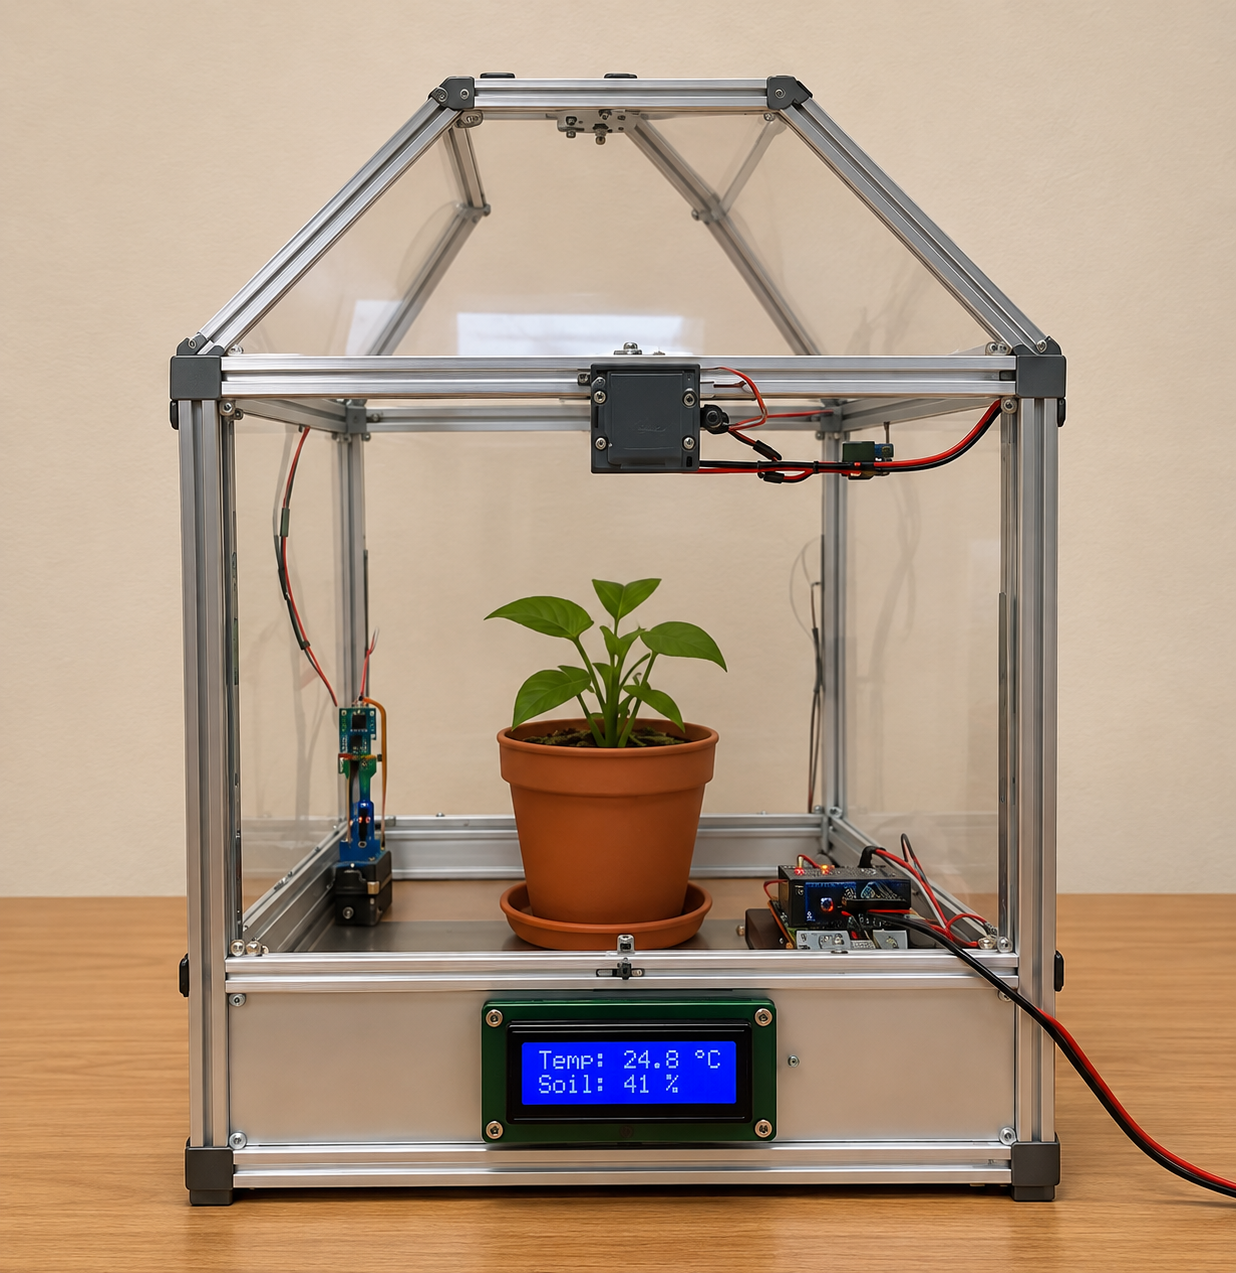
\includegraphics[height=7.2cm]{greenhouse.png}\par
  \vspace{0.9cm}
  \begin{tabular}{@{}l@{\hspace{2.5cm}}l@{}}
    \sffamily\bfseries Work done by: & \sffamily\bfseries Supervised by: \\[0.2em]
    EL AZZOUZI Ayoub   & BELAMFEDEL ALAOUI Sadek \\
    AMMARI Salma       & \\
    BOURICH Yassine    & \\
    HAFIDI Omar        & \\
  \end{tabular}
  \vfill
  {\sffamily UM6P -- College of Computing \quad$\cdot$\quad November 2026\par}
\end{titlepage}

% ------------------------------ ABSTRACT + TOC ------------------------------
\twocolumn[{%
  \begin{center}
  \begin{minipage}{0.9\textwidth}
  \infobox{Abstract}{%
  \emph{Biodome} is a small greenhouse whose soil moisture and air temperature are
  regulated automatically by an Arduino Uno R3. A resistive soil-moisture probe, a
  water-level strip in the reservoir and a type-K thermocouple (read through a MAX6675)
  are the sensors; a DC water pump, a heating resistance and a fan, each switched by a
  relay, are the actuators. A 16$\times$2 LCD with five push buttons shows the live
  measurements and lets the user change every threshold, which is saved in EEPROM.
  We first tried to model the plant with continuous dynamics, then with a hybrid
  automaton, but both needed physical quantities we could not measure precisely with
  our sensors. The final controller is therefore made of two \emph{extended
  finite-state machines} (irrigation and temperature), executed by a small generic
  automaton engine written in C++. This report explains the hardware, the modelling
  path and the choices we made, the final automata, the screen interface, and the
  difficulties we met, especially the very sensitive moisture sensor, the inaccurate
  water-level sensor and the fact that every test risked damaging the plant.}
  \end{minipage}
  \end{center}
  \vspace{0.6em}
}]

{\small\tableofcontents}

% =====================================================================
\section{Introduction}
% =====================================================================

\subsection{Context}
Plant growth depends on a few environmental conditions (mainly how wet the soil is and
how warm the air is) that change continuously during the day. In a closed greenhouse
they also change faster than outside: the sun heats the enclosure, and the small
volume of soil in a pot dries quickly. These conditions must therefore be
\emph{monitored} and \emph{corrected} continuously.

\subsection{Problem}
Without automation, keeping the right soil moisture and temperature is manual,
imprecise and inefficient: someone has to check the plant several times a day, guess
how much water to give, and open or heat the greenhouse by hand. Over-watering is as
harmful as forgetting to water, and both are common.

\subsection{Objective}
Design and build an \keyword{embedded controller} that automatically regulates the
irrigation and the temperature of a mini-greenhouse from sensor measurements. The
system had to:
\begin{enumerate}
  \item measure the soil moisture, the air temperature and the water left in the tank;
  \item water the plant when the soil is too dry, without flooding it;
  \item heat when it is too cold and ventilate when it is too hot;
  \item never run the pump dry, and switch everything off safely when a sensor fails;
  \item show the measurements on a screen and let the user change the thresholds
        without re-programming the board;
  \item be described by a clear, verifiable \keyword{model} (an automaton) rather than
        by ad-hoc \code{if} statements.
\end{enumerate}

\begin{figure}[t]
  \centering
  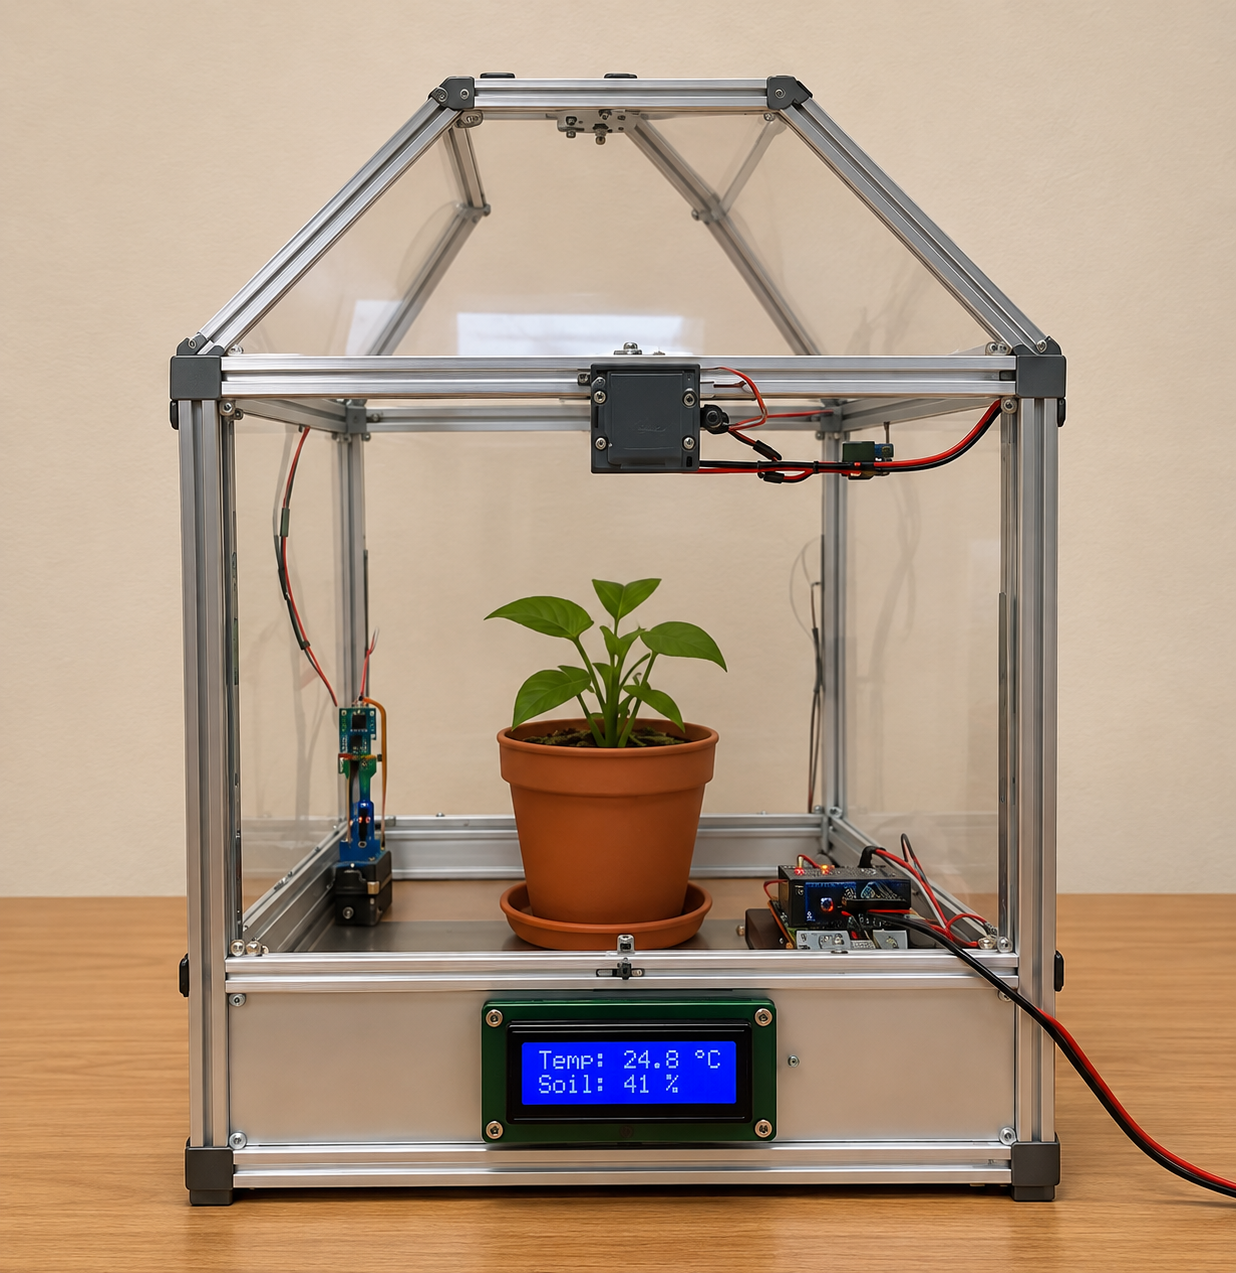
\includegraphics[width=0.78\columnwidth]{greenhouse.png}
  \caption{The Biodome prototype: aluminium-profile enclosure, the plant, and the
  LCD showing the live measurements at the front.}
  \label{fig:greenhouse}
\end{figure}

\subsection{Report outline}
Section~\ref{sec:hardware} presents the physical components and the system
architecture. Section~\ref{sec:modeling} explains the modelling approaches we tried
and why we abandoned them. Section~\ref{sec:final} describes the final model, two
extended finite-state machines, and Section~\ref{sec:software} its implementation.
Section~\ref{sec:screen} presents the screen and the menus. Section~\ref{sec:difficulties}
lists the difficulties we met and how we dealt with them, and
Section~\ref{sec:conclusion} concludes.

% =====================================================================
\section{Hardware and system architecture}\label{sec:hardware}
% =====================================================================

\subsection{Overview}
The system follows the classic \emph{sense -- decide -- act} structure
(Fig.~\ref{fig:architecture}). Sensors and buttons are inputs of the Arduino Uno; the
LCD and three relays are its outputs; the relays switch the power actuators. The water
goes from the reservoir to the plant through silicone tubing, pushed by the pump.

\begin{figure*}[t]
  \centering
  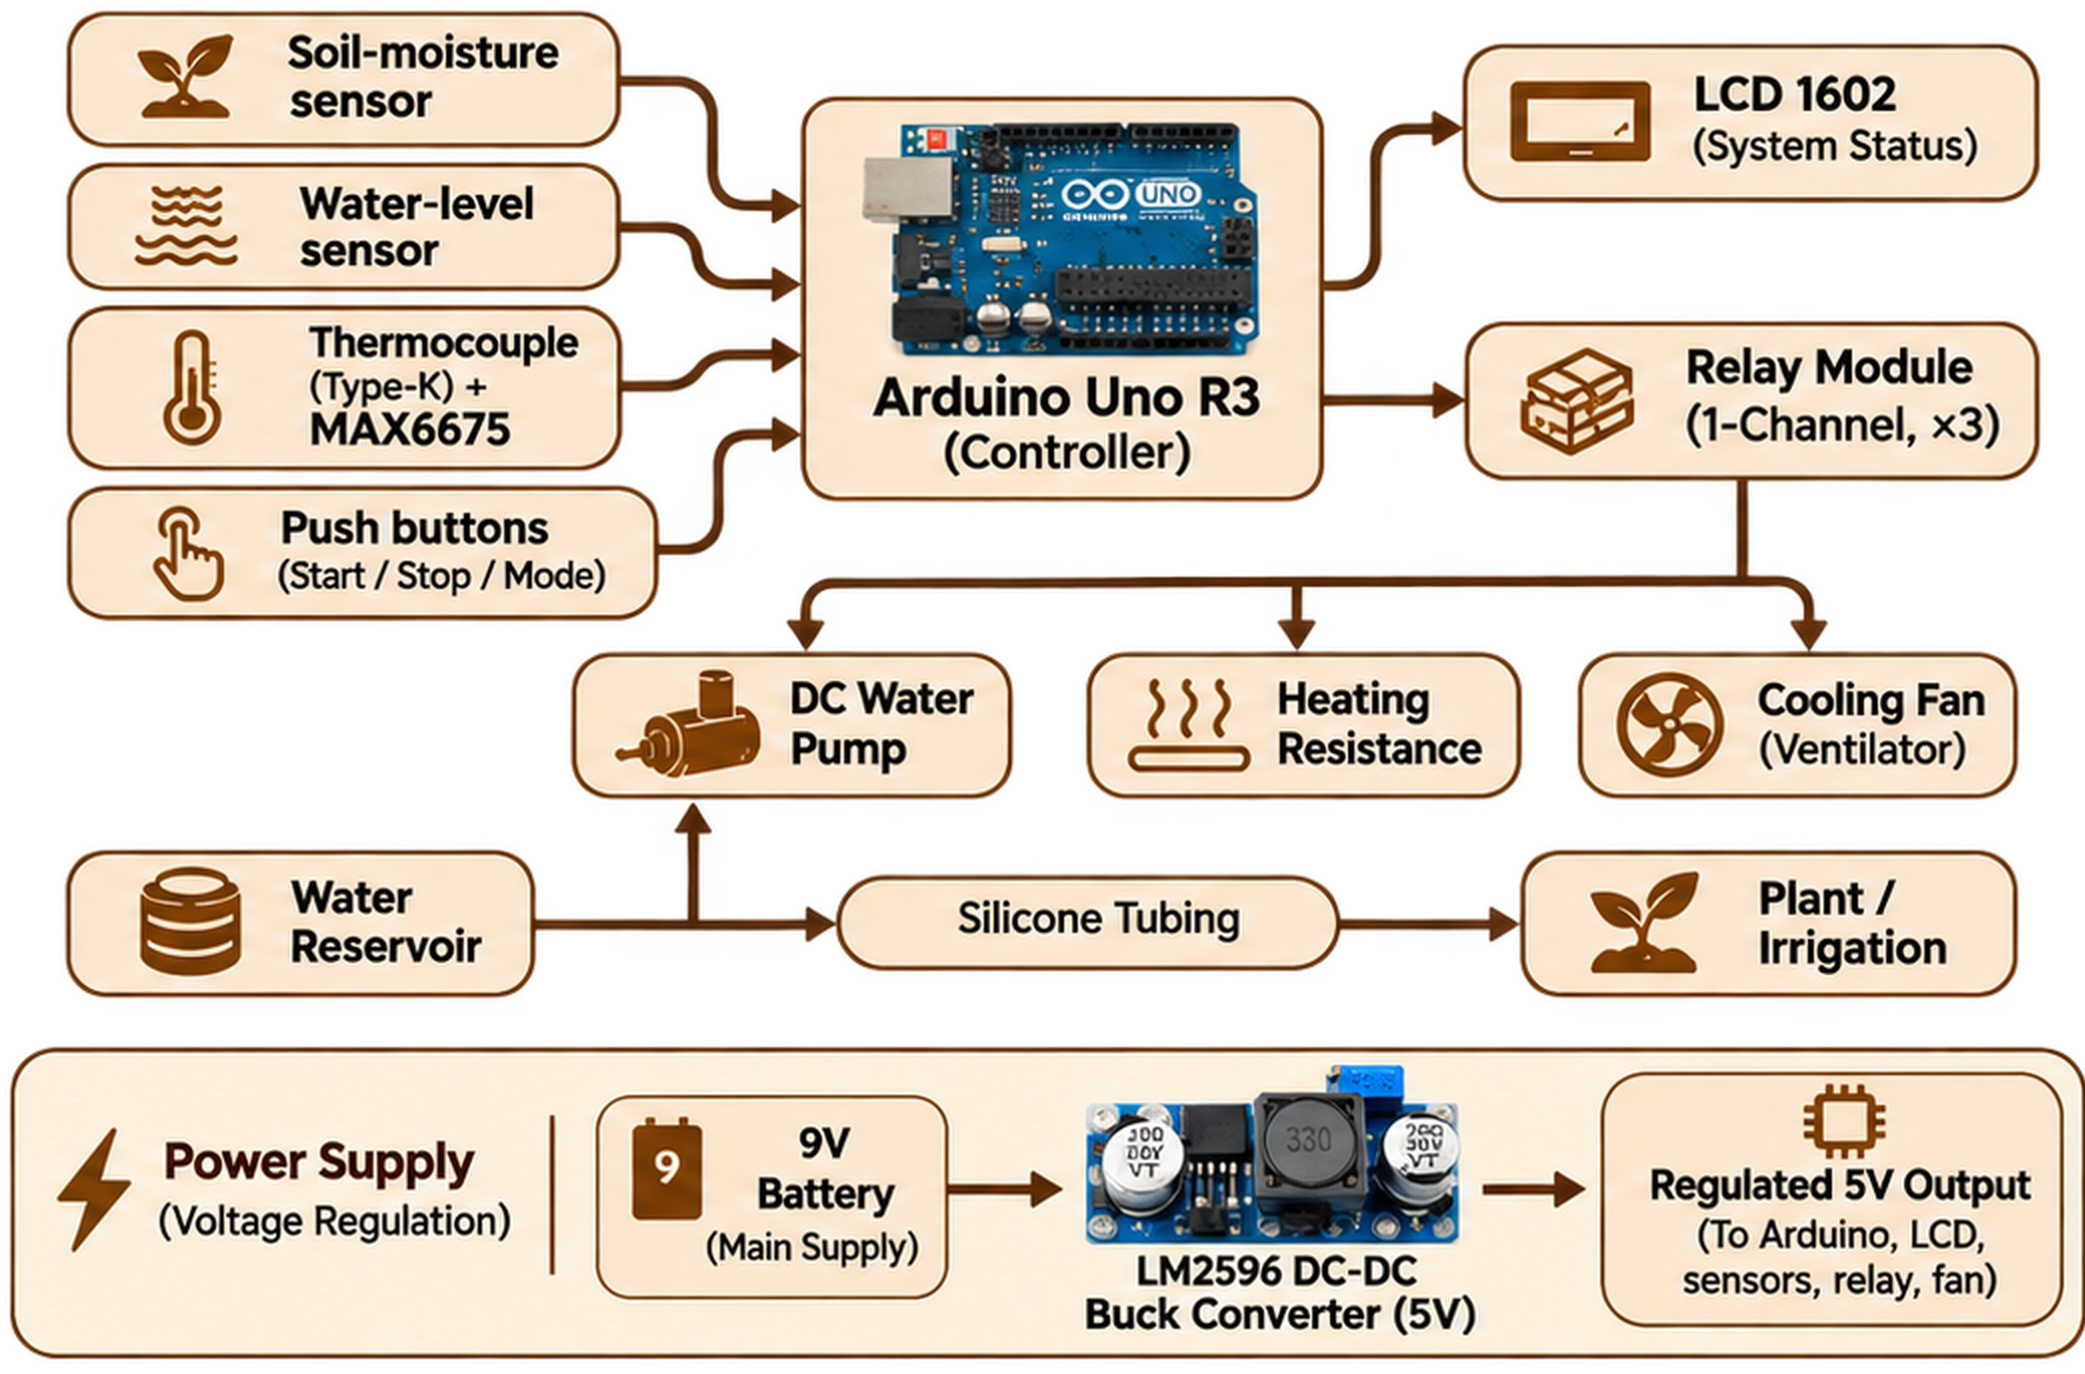
\includegraphics[width=0.82\textwidth]{architecture.png}
  \caption{System architecture. Inputs (left) are read by the Arduino Uno R3, which
  drives the LCD and three 1-channel relays; the relays switch the pump, the heating
  resistance and the fan. The power stage regulates the battery voltage to 5\,V.}
  \label{fig:architecture}
\end{figure*}

\subsection{Components}
Fig.~\ref{fig:hardware} groups the components we used into five families, and
Table~\ref{tab:components} gives the full list with the role of each part. The list
was prepared at the start of the project; some parts
were ordered in more copies than needed, as spares.

\begin{figure}[t]
  \centering
  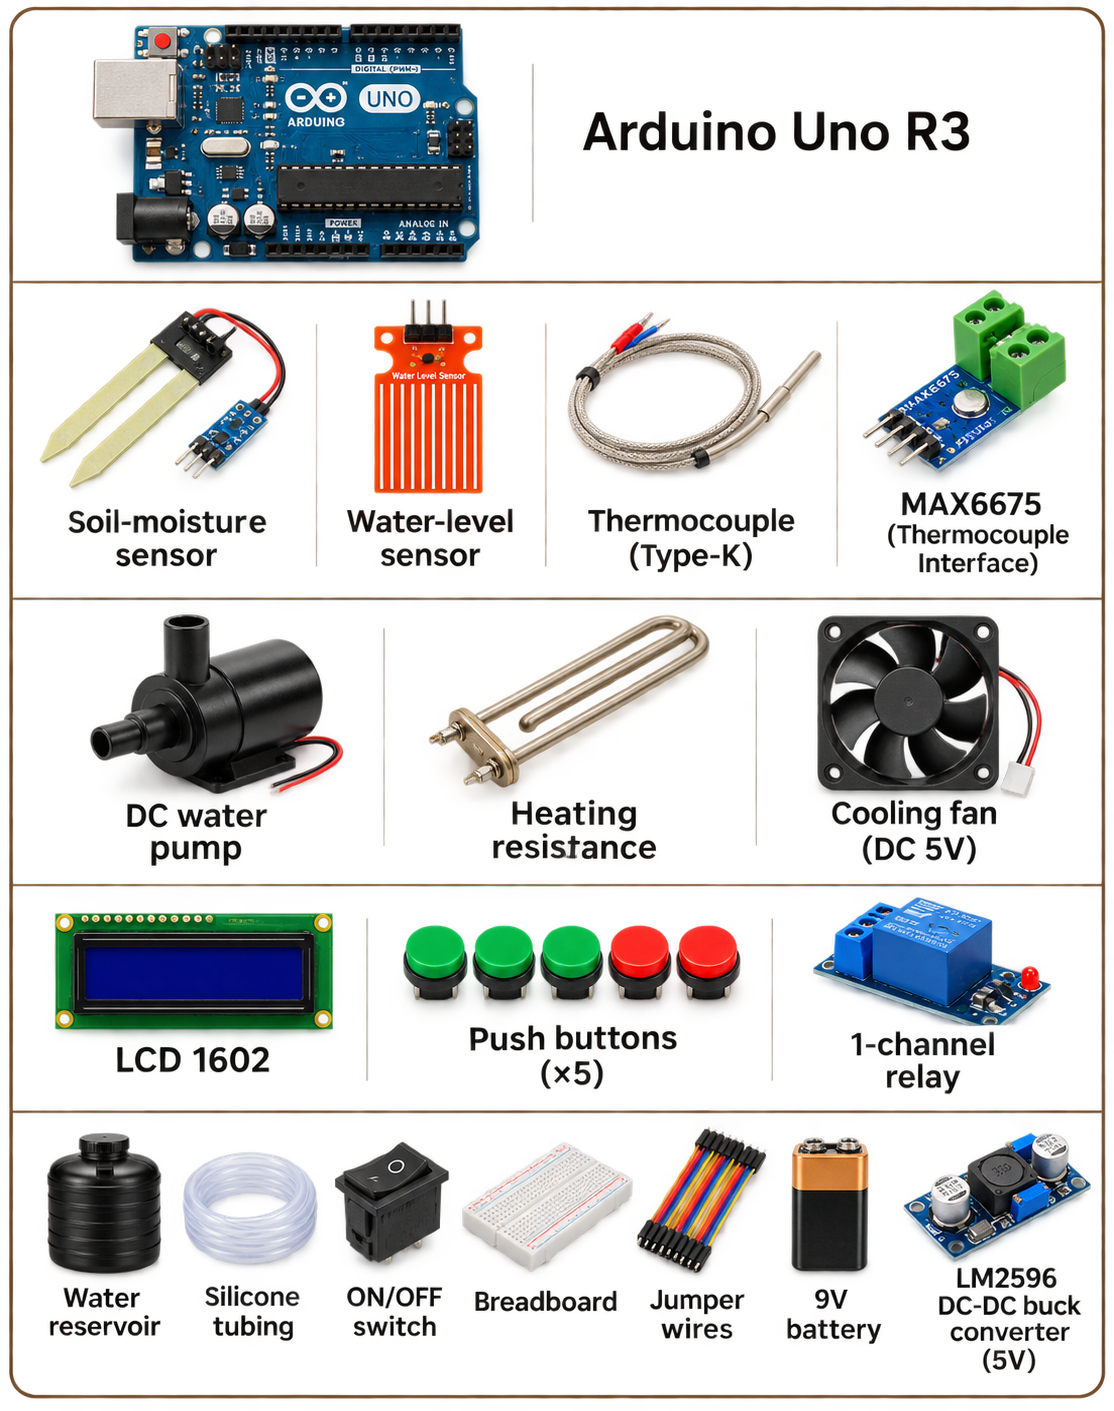
\includegraphics[width=0.92\columnwidth]{hardware.png}
  \caption{Hardware used, by family: controller, sensors, actuators, interface and
  switching, and support (water, power, wiring).}
  \label{fig:hardware}
\end{figure}

\begin{table*}[t]
\centering\small
\caption{Bill of materials. \emph{Qty} is the quantity on our component list; the
last column is how many are used in the final build.}
\label{tab:components}
\begin{tabularx}{\textwidth}{@{}c l l X c c@{}}
\toprule
\# & Component & Family & Role in the project & Qty & Used\\
\midrule
1  & Arduino Uno R3 & Controller & ATmega328P, 16\,MHz, 32\,KB flash, 2\,KB RAM, 1\,KB EEPROM. Runs the automata and the menu. & 1 & 1\\
2  & Soil-moisture sensor (resistive fork) & Sensor & Measures soil moisture on A0; powered only while read (D7). & 4 & 1\\
3  & Water-level sensor (resistive strip) & Sensor & Detects whether the reservoir still has water (A1, powered by A2). & 1 & 1\\
4  & Thermocouple type K & Sensor & Air temperature inside the greenhouse (0--600\,$^\circ$C range, 1\,m cable). & 2 & 1\\
5  & MAX6675 module & Sensor interface & Cold-junction compensation + 12-bit ADC, read over SPI (0.25\,$^\circ$C resolution). & 3 & 1\\
6  & DC water pump & Actuator & Pumps water from the reservoir to the plant. & 1 & 1\\
7  & Heating resistance & Actuator & Heats the air when the temperature is too low. & 1 & 1\\
8  & Fan (5\,V DC) & Actuator & Cools / renews the air; also spreads heat while heating. & 1 & 1\\
9  & 1-channel relay module & Switching & One per actuator: pump (D10), heater (D9), fan (D8). & 4 & 3\\
10 & Silicone tubing (1.5\,m) & Support & Carries water from the pump to the pot. & 1 & 1\\
11 & Water reservoir & Support & Holds the irrigation water; contains the level sensor. & 1 & 1\\
12 & ON/OFF switch & Support & Main power switch. & 1 & 1\\
13 & LCD 1602 + I\textsuperscript{2}C backpack & Interface & Live metrics and menus (SDA = A4, SCL = A5). & 1 & 1\\
14 & Push buttons & Interface & MENU, OK, CANCEL, UP, DOWN (D2--D6, to GND). & 6 & 5\\
15 & Jumper wires & Support & Wiring on the breadboard. & 25 & --\\
16 & Breadboard & Support & Prototype wiring. & 1 & 1\\
17 & Batteries (9\,V, 3.7\,V cells + holder) & Power & Main supply. & -- & --\\
18 & Regulator (LM2596 DC-DC buck) & Power & Regulated 5\,V output for the Arduino, LCD, sensors, relays and fan. & 1 & 1\\
\bottomrule
\end{tabularx}
\end{table*}


\subsection{Sensors}
\paragraph{Soil-moisture sensor.} A resistive fork: the two metal legs form a
resistance whose value drops when the soil is wet; the small comparator board outputs
an analog voltage (0--1023 on the 10-bit ADC; \emph{higher = drier}). It is calibrated
with two points: the raw value in dry air ($\mathit{raw}_{dry}=850$) and in a glass of
water ($\mathit{raw}_{wet}=140$), and converted to a percentage:
\begin{equation}
  H\,[\%] = \operatorname{clamp}_{[0,100]}
  \left(\operatorname{round}\!\left(100\,\frac{\mathit{raw}_{dry}-\mathit{raw}}
  {\mathit{raw}_{dry}-\mathit{raw}_{wet}}\right)\right).
  \label{eq:calib}
\end{equation}
A DC current through the legs corrodes them by electrolysis, so the probe is
\emph{powered only while it is read} (pin D7 HIGH for 100\,ms every 2\,s).

\paragraph{Water-level sensor.} A strip of parallel copper tracks placed in the
reservoir: the more tracks are under water, the higher the output. It is used
\emph{only as a binary safety signal} (tank \emph{OK} / tank \emph{empty}) compared to
an adjustable threshold, because its readings were too inaccurate to give a real level
(Section~\ref{sec:difficulties}). It is powered from A2 (used as a digital output),
also only while being read.

\paragraph{Thermocouple + MAX6675.} A type-K thermocouple measures the air temperature;
the MAX6675 converter compensates the cold junction and sends a 12-bit value over a
3-wire SPI bus (SCK = D13, CS = D12, SO = D11). A conversion takes about 220\,ms, so it
is never read faster than every 250\,ms. The module also reports when the probe is
disconnected, which we use as a fault signal.

\subsection{Actuators and switching}
The \textbf{pump}, the \textbf{heating resistance} and the \textbf{fan} cannot be
supplied by an Arduino pin (40\,mA max), so each one is switched by a 1-channel relay
module driven by a digital pin. All three are \emph{on/off} actuators: this binary
nature turned out to be decisive for the choice of the model
(Section~\ref{sec:modeling}). Because some relay modules are active-low, the ON/OFF
levels of each actuator are defined by one macro (\code{PUMP\_ON}, \code{FAN\_ON},
\dots) and can be inverted in one line.

\subsection{Interface}
A 16$\times$2 LCD with an I\textsuperscript{2}C backpack only uses the two
I\textsuperscript{2}C pins (A4, A5), which leaves enough pins for the five buttons.
Each button is wired between its pin and GND and uses the internal pull-up resistor
(\code{INPUT\_PULLUP}), so no external resistor is needed (Fig.~\ref{fig:buttons}).

\begin{figure}[t]
  \centering
  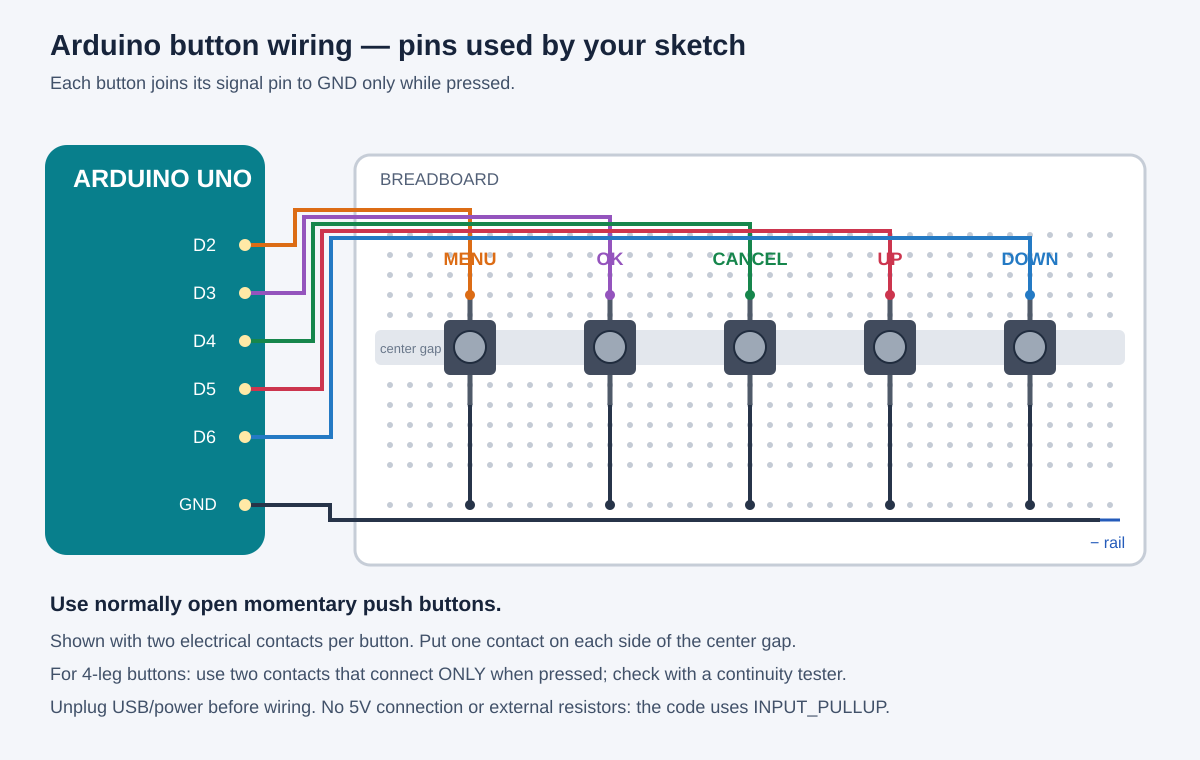
\includegraphics[width=\columnwidth]{button_wiring.png}
  \caption{Button wiring: each push button goes from its digital pin (D2--D6) to GND,
  with the internal pull-up enabled (released = HIGH, pressed = LOW).}
  \label{fig:buttons}
\end{figure}

\subsection{Power supply}
The main supply is a battery pack. An LM2596 DC-DC buck converter regulates it down
to a stable 5\,V, which feeds the Arduino, the LCD, the sensors, the relay modules and
the fan. A buck converter was chosen instead of a linear regulator because it wastes
much less energy as heat, which matters on batteries. A main ON/OFF switch cuts the
whole system.

\subsection{Pin assignment}
Table~\ref{tab:pins} summarises the wiring, exactly as defined in the code.

\begin{table}[h]
\centering\small
\caption{Arduino Uno pin assignment.}
\label{tab:pins}
\begin{tabularx}{\columnwidth}{@{}l l X@{}}
\toprule
Pin & Direction & Connected to \\
\midrule
A0 & analog in & soil-moisture sensor (signal) \\
A1 & analog in & water-level sensor (signal) \\
D7 & out & soil-moisture sensor power \\
A2 & out & water-level sensor power \\
D13 / D12 / D11 & SPI & MAX6675 SCK / CS / SO \\
D10 & out & relay: pump \\
D9 & out & relay: heating resistance \\
D8 & out & relay: fan \\
D2 / D3 / D4 & in (pull-up) & MENU / OK / CANCEL \\
D5 / D6 & in (pull-up) & UP / DOWN \\
A4 / A5 & I\textsuperscript{2}C & LCD SDA / SCL \\
\bottomrule
\end{tabularx}
\end{table}

\subsection{Physical build}
The electronics are wired on a breadboard on a
tray: the Arduino on the left, the LM2596 converter and the power switch at the bottom,
the MAX6675 module and the sensor boards at the top, and the three relay modules on
the right. The tray sits outside the growing area so that water cannot reach the
electronics.


% =====================================================================
\section{Modelling approaches and design choices}\label{sec:modeling}
% =====================================================================
Before writing the controller we wanted a \emph{model} of the greenhouse, to reason
about the behaviour instead of tuning by trial and error. We went through three
models before reaching the final one; each step taught us something.

\subsection{First attempt: continuous dynamics}
Using what we knew from continuous modelling, we tried to describe the physical
quantities with differential equations and transfer functions
(Fig.~\ref{fig:continuous}). Let $V$ be the pore volume of the soil, $w(t)\in[0,V]$
the water it contains, $p(t)\in[0,1]$ the pump power and $r$ the maximal water rate of
the pump. Then
\begin{equation}
  \dot w(t) = r\,p(t), \qquad m(t)=\frac{w(t)}{V}\in[0,1].
\end{equation}
If the pump runs at full power from the measurement instant $t_0$,
$m(t)-m(t_0)=\frac{r}{V}(t-t_0)$, and in the Laplace domain the moisture is a pure
integrator of the pump command:
\begin{equation}
  M(s) = \frac{r}{V}\,\frac{1}{s}\,P(s).
\end{equation}

\begin{figure}[t]
  \centering
  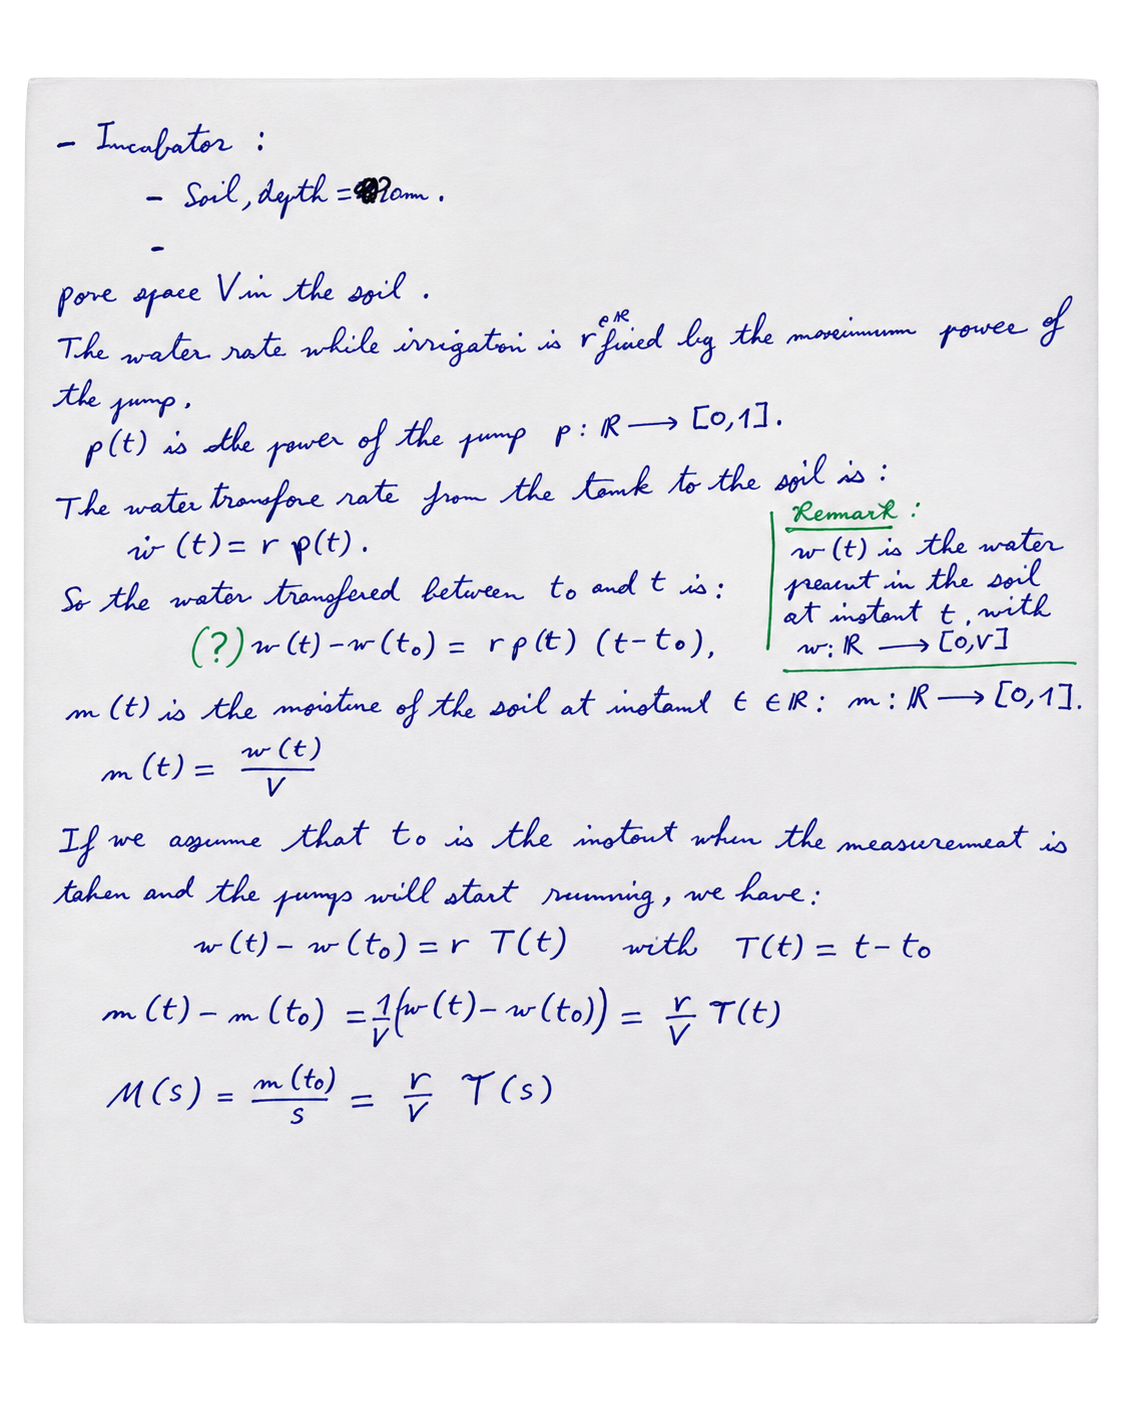
\includegraphics[width=0.85\columnwidth]{continuous_model.png}
  \caption{Our first, continuous model of the irrigation (hand-written notes).}
  \label{fig:continuous}
\end{figure}

We also wrote a first sketch with a \textbf{discrete proportional controller}: every
period $T$ (60\,s) the moisture $M_k$ is measured and the pump runs for
$u_k = K_p\,(M_{ref}-M_k)$ seconds, clamped to $[0,U_{max}]$. With the simple model
$M_{k+1}=M_k+b\,u_k$ ($b$ = \% of moisture gained per second of pumping), the error
obeys $e_{k+1}=(1-bK_p)\,e_k$, which is stable if and only if
\begin{equation}
  |1-bK_p|<1 \iff 0<K_p<\frac{2}{b}.
\end{equation}
The sketch had test modes to check the wiring, to calibrate the sensor and to measure
$b$ (read $M$, pump for 3\,s, wait 60\,s for the water to soak, read again).

\infobox{Why we abandoned it}{%
\begin{itemize}[leftmargin=1em]
  \item The actuators are \emph{purely discrete}: the pump, the heater and the fan are
        either ON or OFF through a relay; $p(t)\in[0,1]$ does not exist in reality.
  \item The model ignores evaporation, drainage and the time the water takes to
        spread in the soil, which dominate the real behaviour.
  \item The parameters ($r$, $V$, $b$) could not be measured reliably: the moisture
        sensor jumps as soon as a drop touches it, and every identification run
        soaks the soil (Section~\ref{sec:difficulties}).
\end{itemize}}

\subsection{Second attempt: hybrid automaton}
Since the actuators are discrete but the moisture still evolves continuously, the
natural next step was a \keyword{hybrid automaton} (Fig.~\ref{fig:hybrid}): discrete
modes (\emph{Idle}, \emph{Irrigating}, \emph{Fault}) each with its own flow,
\begin{equation}
  \dot H = \alpha\,u_p - \beta, \qquad u_p\in\{0,1\},
\end{equation}
where $\alpha$ is the moisture gain rate of the pump and $\beta$ the drying rate; and
guards on the moisture ($H\le H_{low}$, $H\ge H_{target}$) and on clocks
($s_c\ge T_{cool}$, $s_p\ge T_{max}$).

\begin{figure}[t]
  \centering
  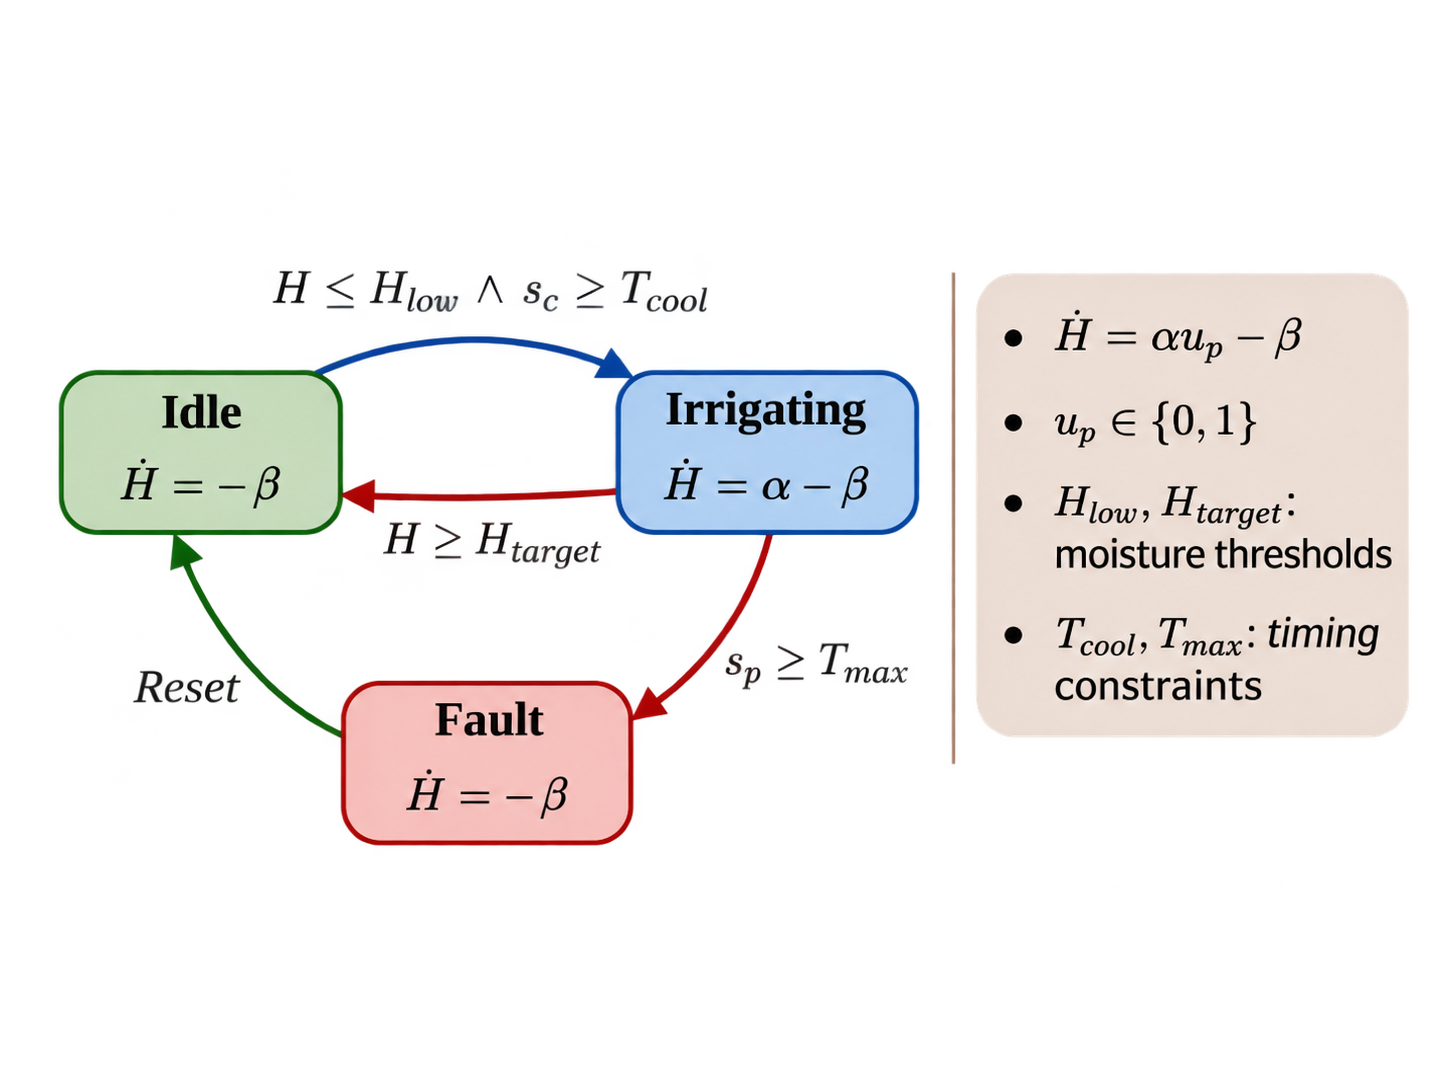
\includegraphics[width=\columnwidth]{hybrid_automaton.png}
  \caption{The hybrid automaton we designed for the irrigation: each mode has a flow
  $\dot H$, transitions are guarded by moisture thresholds and timers.}
  \label{fig:hybrid}
\end{figure}

\infobox{Why we abandoned it}{%
The structure (modes, guards, timers) was right, but the \emph{flows} were not usable:
even with relaxation we could not obtain reasonable values for $\alpha$ and $\beta$.
They depend on the soil, the pot, the temperature, the evaporation and, above all, on a
sensor that is not precise enough to measure a rate. A model whose main parameters are
guesses does not let us prove anything.}

\subsection{The decision: extended finite-state machines}
The two attempts showed what really matters: the \emph{discrete} decisions (when to
switch each actuator ON or OFF), the \emph{thresholds} on the measurements, and a few
\emph{timing constraints}. We therefore kept the discrete skeleton of the hybrid
automaton, dropped the continuous flows, and moved the timers and the measurements
into the guards. The result is an \keyword{extended finite-state machine} (EFSM):
\begin{itemize}
  \item it needs no physical parameter: only thresholds, which the user can set
        on the screen and correct by observation;
  \item it matches the hardware: every output is a function of the current state
        (pump ON $\iff$ state \emph{IRRIGATING});
  \item it is small, deterministic, and easy to check exhaustively by hand;
  \item it runs in constant time and memory on a 2\,KB-RAM microcontroller.
\end{itemize}

% =====================================================================
\section{Final model: extended finite-state machines}\label{sec:final}
% =====================================================================

\subsection{Definition}
Each controller is a tuple $\mathcal{A}=(Q,\,q_0,\,X,\,\Delta,\,\lambda)$ where
\begin{itemize}
  \item $Q$ is a finite set of states and $q_0\in Q$ the initial state;
  \item $X$ are the \emph{extended variables}: the last measurements
        ($H$, $T$, \textit{tankOK}), the thresholds, and timestamps
        ($t_{on}$, $t_{off}$, $t_{th}$) compared with the clock $\mathit{now}$;
  \item $\Delta$ is an \emph{ordered} list of transitions
        $q\xrightarrow{[g]\,/\,a}q'$ with a guard $g$ (a predicate over $X$) and an
        optional action $a$ (an update of $X$, typically saving $\mathit{now}$);
  \item $\lambda:Q\to\{0,1\}^k$ gives the actuator outputs (Moore machine).
\end{itemize}
At each step, the automaton evaluates the guards of the transitions leaving the
current state \emph{in their order of priority} and fires the first one that is
enabled (at most one transition per step). This order makes the machine
\textbf{deterministic} even when two guards are true at the same time, and we always
put the \textbf{safety transitions first}.

The automaton itself contains no clock and no continuous dynamics: anything about time
(\emph{``the pump has run for 2\,s''}) or about measurements (\emph{``moisture
$<35\,\%$''}) is computed in the guards.

\subsection{Irrigation automaton}
States:
\[Q_I=\{\text{IDLE},\,\text{IRRIGATING},\,\text{TANK\_EMPTY}\},\]
initial state IDLE, output $\mathit{pump}=1 \iff q=\text{IRRIGATING}$ (Fig.~\ref{fig:irrigation},
Table~\ref{tab:irrigation}).

\begin{figure*}[t]
\centering
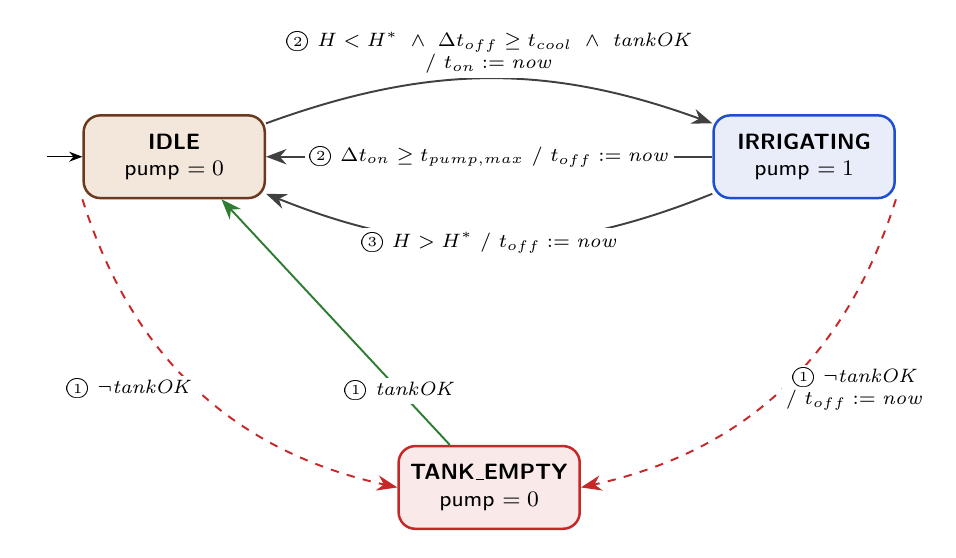
\begin{tikzpicture}[>=Stealth]
  \node[st, initial, initial text={}] (idle) at (0,0) {\textbf{IDLE}\\pump $=0$};
  \node[stact] (irr) at (8,0) {\textbf{IRRIGATING}\\pump $=1$};
  \node[sterr] (empty) at (4,-4.2) {\textbf{TANK\_EMPTY}\\pump $=0$};

  \draw[tr] (idle) to[bend left=20] node[lab, above]
      {\textcircled{\tiny 2} $H<H^{*}\ \wedge\ \Delta t_{off}\ge t_{cool}\ \wedge\ \mathit{tankOK}$\\ $/\ t_{on}:=\mathit{now}$} (irr);
  \draw[tr] (irr) -- node[lab]
      {\textcircled{\tiny 2} $\Delta t_{on}\ge t_{pump,max}\ /\ t_{off}:=\mathit{now}$} (idle);
  \draw[tr] (irr) to[bend left=22] node[lab, pos=0.5]
      {\textcircled{\tiny 3} $H>H^{*}\ /\ t_{off}:=\mathit{now}$} (idle);
  \draw[safe] (idle.south west) to[bend right=30] node[lab, left, pos=0.5]
      {\textcircled{\tiny 1} $\neg\mathit{tankOK}$} (empty.west);
  \draw[safe] (irr.south east) to[bend left=30] node[lab, right, pos=0.5]
      {\textcircled{\tiny 1} $\neg\mathit{tankOK}$\\$/\ t_{off}:=\mathit{now}$} (empty.east);
  \draw[tr, draw=okgreen] ([xshift=-5mm]empty.north) -- node[lab, pos=0.22]
      {\textcircled{\tiny 1} $\mathit{tankOK}$} ([xshift=6mm]idle.south);
\end{tikzpicture}
\caption{Irrigation automaton. $H$ = soil moisture (\%), $H^*$ = target moisture
(\code{H\_TARGET}), $\Delta t_{on}=\mathit{now}-t_{on}$, $\Delta t_{off}=\mathit{now}-t_{off}$.
Circled numbers give the priority among the transitions leaving the same state; red
dashed arrows are the safety transitions (always tried first).}
\label{fig:irrigation}
\vspace{0.9em}
\small
\captionof{table}{Transitions of the irrigation automaton, in the order they are tried.}
\label{tab:irrigation}
\begin{tabularx}{\textwidth}{@{}c l l l l X@{}}
\toprule
Prio & From & To & Guard (code) & Action & Meaning\\
\midrule
1 & IDLE & TANK\_EMPTY & \code{tankEmpty()} & -- & never start the pump without water\\
2 & IDLE & IRRIGATING & \code{soilDry()} & \code{startPump()} & $H^*>0$, $H<H^*$, cool-down elapsed, tank OK\\
1 & IRRIGATING & TANK\_EMPTY & \code{tankEmpty()} & \code{stopPump()} & tank ran out while watering\\
2 & IRRIGATING & IDLE & \code{pumpTooLong()} & \code{stopPump()} & one watering pulse is over ($t_{pump,max}$, default 2\,s)\\
3 & IRRIGATING & IDLE & \code{soilWet()} & \code{stopPump()} & the soil is already wet enough\\
1 & TANK\_EMPTY & IDLE & \code{tankRefilled()} & -- & the reservoir was refilled\\
\bottomrule
\end{tabularx}
\end{figure*}

\paragraph{Watering by pulses.} The pump never runs ``until the soil is wet'': water
takes minutes to spread in the soil, while the sensor reacts immediately to the water
that touches it. If we waited for $H$ to rise, we would flood the pot. Instead, the
automaton gives a short \textbf{pulse} (2\,s by default), then waits for a
\textbf{cool-down} (15\,min by default) before it looks at the moisture again. The
cool-down plays the role of a hysteresis in \emph{time} and prevents the pump from
chattering around $H^*$. Setting $H^*=0$ disables watering completely.

\subsection{Temperature automaton}
States:
\[\begin{aligned}Q_T=\{&\text{IDLE},\,\text{HEATING},\\&\text{COOLING},\,\text{SENSOR\_ERROR}\},\end{aligned}\]
initial state IDLE (Fig.~\ref{fig:temperature}, Table~\ref{tab:temperature}).
Outputs: $\mathit{heater}=1\iff q=\text{HEATING}$, and $\mathit{fan}=1\iff
q\in\{\text{HEATING},\text{COOLING}\}$: the fan also runs while heating, to spread the
warm air in the enclosure.

\begin{figure*}[t]
\centering
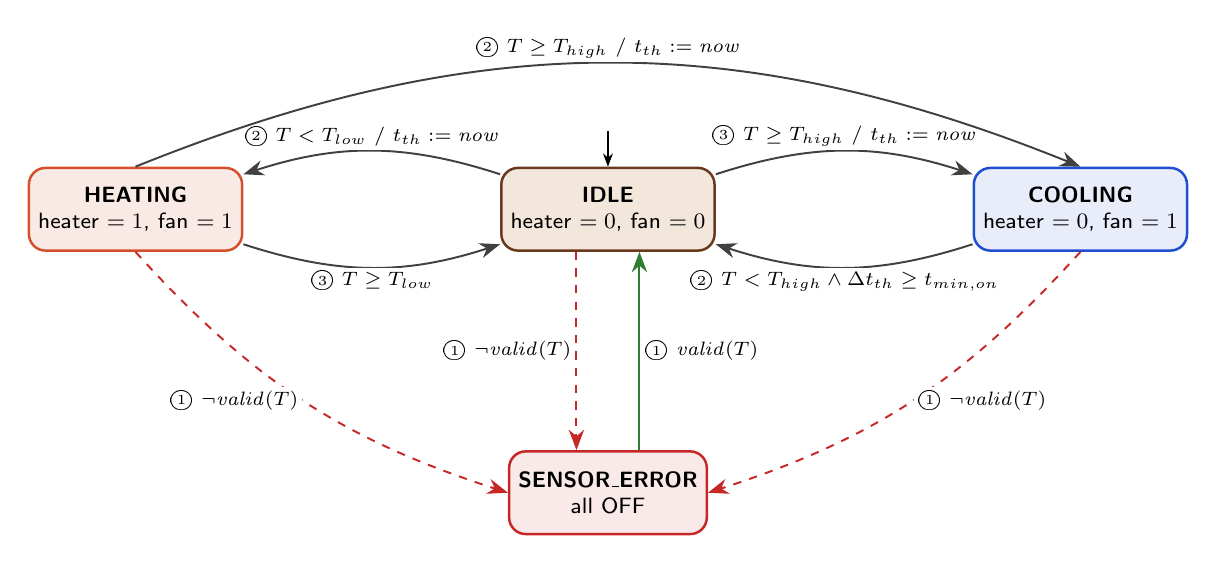
\begin{tikzpicture}[>=Stealth]
  \node[st, initial above, initial text={}] (idle) at (0,0) {\textbf{IDLE}\\heater $=0$, fan $=0$};
  \node[stact, fill=accent!12, draw=accent] (heat) at (-6,0) {\textbf{HEATING}\\heater $=1$, fan $=1$};
  \node[stact] (cool) at (6,0) {\textbf{COOLING}\\heater $=0$, fan $=1$};
  \node[sterr] (err) at (0,-3.6) {\textbf{SENSOR\_ERROR}\\all OFF};

  \draw[tr] (idle) to[bend right=18] node[lab, above] {\textcircled{\tiny 2} $T<T_{low}\ /\ t_{th}:=\mathit{now}$} (heat);
  \draw[tr] (heat) to[bend right=18] node[lab, below] {\textcircled{\tiny 3} $T\ge T_{low}$} (idle);
  \draw[tr] (idle) to[bend left=18] node[lab, above] {\textcircled{\tiny 3} $T\ge T_{high}\ /\ t_{th}:=\mathit{now}$} (cool);
  \draw[tr] (cool) to[bend left=18] node[lab, below] {\textcircled{\tiny 2} $T<T_{high}\wedge \Delta t_{th}\ge t_{min,on}$} (idle);
  \draw[tr] (heat.north) to[bend left=22] node[lab, above] {\textcircled{\tiny 2} $T\ge T_{high}\ /\ t_{th}:=\mathit{now}$} (cool.north);

  \draw[safe] (heat.south) to[bend right=15] node[lab, left] {\textcircled{\tiny 1} $\neg\mathit{valid}(T)$} (err.west);
  \draw[safe] (cool.south) to[bend left=15] node[lab, right] {\textcircled{\tiny 1} $\neg\mathit{valid}(T)$} (err.east);
  \draw[safe] ([xshift=-4mm]idle.south) -- node[lab, left] {\textcircled{\tiny 1} $\neg\mathit{valid}(T)$} ([xshift=-4mm]err.north);
  \draw[tr, draw=okgreen] ([xshift=4mm]err.north) -- node[lab, right] {\textcircled{\tiny 1} $\mathit{valid}(T)$} ([xshift=4mm]idle.south);
\end{tikzpicture}
\caption{Temperature automaton. $T$ = air temperature, $T_{low}$/$T_{high}$ = heating
and cooling thresholds, $\Delta t_{th}=\mathit{now}-t_{th}$, $t_{min,on}$ = minimum
cooling time. Any invalid reading (no communication, probe disconnected, all-zero data)
sends the automaton to SENSOR\_ERROR from every state, which switches every thermal
actuator off.}
\label{fig:temperature}
\vspace{0.9em}
\small
\captionof{table}{Transitions of the temperature automaton, in the order they are tried.}
\label{tab:temperature}
\begin{tabularx}{\textwidth}{@{}c l l l l X@{}}
\toprule
Prio & From & To & Guard (code) & Action & Meaning\\
\midrule
1 & IDLE & SENSOR\_ERROR & \code{tempInvalid()} & -- & no valid temperature: do nothing blind\\
2 & IDLE & HEATING & \code{tooCold()} & \code{startThermal()} & $T<T_{low}$ (default 18\,$^\circ$C)\\
3 & IDLE & COOLING & \code{tooHot()} & \code{startThermal()} & $T\ge T_{high}$ (default 28\,$^\circ$C)\\
1 & HEATING & SENSOR\_ERROR & \code{tempInvalid()} & -- & sensor lost while heating: heater OFF\\
2 & HEATING & COOLING & \code{tooHot()} & \code{startThermal()} & overshoot: go straight to cooling\\
3 & HEATING & IDLE & \code{warmEnough()} & -- & $T\ge T_{low}$\\
1 & COOLING & SENSOR\_ERROR & \code{tempInvalid()} & -- & sensor lost while cooling\\
2 & COOLING & IDLE & \code{coolEnough()} & -- & $T<T_{high}$ and the fan ran at least $t_{min,on}$ (60\,s)\\
1 & SENSOR\_ERROR & IDLE & \code{tempValid()} & -- & the sensor works again\\
\bottomrule
\end{tabularx}
\end{figure*}

\paragraph{Hysteresis.} Two mechanisms prevent rapid ON/OFF switching when the
temperature fluctuates around a threshold: (i) the \textbf{band} between $T_{low}$ and
$T_{high}$ (10\,$^\circ$C by default) where nothing is done, so heating and cooling can
never fight each other, and (ii) the \textbf{minimum ON time} of the fan in COOLING,
which stops it from toggling every sample around $T_{high}$. Heating stops as soon as
$T_{low}$ is reached; its switching rate is limited by the 2\,s sampling period.

\subsection{Properties checked by inspection}
Because the automata are small, we checked these properties by going through every
state and transition:
\begin{enumerate}
  \item \textbf{No dry pumping:} the pump output requires $q=\text{IRRIGATING}$
        \emph{and} \textit{tankOK}; any transition into IRRIGATING requires
        \textit{tankOK}, and $\neg$\textit{tankOK} has the highest priority in
        IRRIGATING.
  \item \textbf{Bounded watering:} every stay in IRRIGATING lasts at most
        $t_{pump,max}$ plus one loop iteration, and two pulses are separated by at
        least $t_{cool}$.
  \item \textbf{No heater/fan conflict:} the heater is ON only in HEATING, and
        heating and cooling are exclusive states.
  \item \textbf{Fail-safe:} an invalid temperature reaches SENSOR\_ERROR from every
        state in one step; all thermal outputs are OFF there.
  \item \textbf{Determinism:} transitions leaving a state are totally ordered, and at
        most one transition fires per step.
\end{enumerate}

% =====================================================================
\section{Software implementation}\label{sec:software}
% =====================================================================

\subsection{Code organisation}
The code is split into small modules:
\begin{description}[leftmargin=0.6em,style=nextline,itemsep=0.2em]
  \item[\code{Model.h}] abstract interface with \code{init()} and \code{run()}.
  \item[\code{Automaton.h/.cpp}] a generic EFSM engine (states, guarded transitions,
        actions), independent of the greenhouse.
  \item[\code{Settings.h/.cpp}] all thresholds, defaults, validation and EEPROM storage.
  \item[\code{Menu.h/.cpp}] LCD, buttons, live metrics and threshold editor.
  \item[\code{GreenhouseSimple.ino}] pins, sensor reading, the two automata
        (guards, actions, transition tables), and the main loop.
  \item[\code{WaterLevelTest.ino}] a stand-alone diagnostic sketch for the
        water-level sensor.
\end{description}

\subsection{The automaton engine}
Guards and actions are plain function pointers (\code{bool (*)()} and
\code{void (*)()}). The Uno has no \code{std::unordered\_map} and dynamic memory is
risky with 2\,KB of RAM, so all tables are fixed-size arrays. States are small
integers, so an array indexed by the state works as a perfect hash map: for each state
we store the index of its first outgoing transition, and the transitions of one state
are chained through a \code{next\_} array. \code{run()} therefore jumps in $O(1)$ to the
current state and only looks at its own transitions, in the order they were added:

\begin{lstlisting}
void Automaton::run() {
  for (byte t = first_[current_]; t != NONE; t = next_[t]) {
    Transition& tr = transitions_[t];
    if (!tr.guard || tr.guard()) {  // no guard = always enabled
      if (tr.action) tr.action();
      current_ = tr.to;
      return;                       // one transition per run()
    }
  }
  // no enabled transition: stay in the current state
}
\end{lstlisting}

The greenhouse automata are then just declared in \code{setup()}; the order of the
calls is the priority order:

\begin{lstlisting}
irrigation.addTransition(IDLE, TANK_EMPTY, tankEmpty, nullptr);
irrigation.addTransition(IDLE, IRRIGATING, soilDry, startPump);
irrigation.addTransition(IRRIGATING, TANK_EMPTY, tankEmpty, stopPump);
irrigation.addTransition(IRRIGATING, IDLE, pumpTooLong, stopPump);
irrigation.addTransition(IRRIGATING, IDLE, soilWet, stopPump);
irrigation.addTransition(TANK_EMPTY, IDLE, tankRefilled, nullptr);
\end{lstlisting}

Guards read the global measurements and settings, for example:

\begin{lstlisting}
bool soilDry() {
  return settings.H_TARGET > 0 && moisture < settings.H_TARGET
      && millis() - pumpStop >= settings.COOLDOWN_MS && tankOk;
}
bool pumpTooLong() { return millis() - pumpStart >= settings.PUMP_MAX_MS; }
\end{lstlisting}

Time comparisons are always written \code{millis() - start >= duration}, which stays
correct when the 32-bit \code{millis()} counter wraps around after 49.7 days.

\subsection{Main loop}
The loop never blocks, so the buttons, the screen and the time limits stay responsive.
Each iteration:
\begin{enumerate}
  \item resets the \textbf{watchdog} (4\,s): if the program ever freezes, the board
        resets and \code{setup()} switches every actuator OFF;
  \item updates the sensors (non-blocking, see below);
  \item runs each automaton once (at most one transition each) and logs every state
        change on the serial port;
  \item sets each relay from the current states (Moore outputs);
  \item prints a status line when a new sample arrived;
  \item updates the screen and the buttons.
\end{enumerate}

\paragraph{Non-blocking sampling.} Every 2\,s the probes are powered; 100\,ms later
(without \code{delay()}) the moisture and water level are read, the probes are
switched off, and the temperature is read. Each analog channel is read twice and the
first conversion is discarded, because after switching channels the ADC needs one
conversion to settle.

\paragraph{Start-up delay.} After a reset, the automata stay in IDLE for 30\,s with
every actuator OFF, while the sensors, the serial log and the menu already work. This
leaves time to check the readings (and to unplug things) before anything moves.

\subsection{Settings in EEPROM}
All thresholds are grouped in one \code{Settings} structure. The factory defaults are
kept in flash (\code{PROGMEM}) to save RAM. In EEPROM the structure is stored after a
\emph{magic byte} and a \emph{version number}; at start-up the stored values are used
only if both match and the values pass \code{settingsValid()} (e.g.\ $0\le H^*\le100$,
$T_{low}<T_{high}$); otherwise the defaults are restored. \code{EEPROM.update()} only
rewrites bytes that changed, which preserves the EEPROM's limited write endurance.

\subsection{Serial log}
The serial monitor prints one status line per sample and one line per transition,
for example:
\begin{lstlisting}[language={}]
H: 31 % (raw 630) Htarget 35 | water raw 412 min 0 (ok) | T: 23.50 C | irrigation IDLE, temperature IDLE | pump OFF heater OFF fan OFF
# [912.4 s] irrigation: IDLE -> IRRIGATING
# [914.4 s] irrigation: IRRIGATING -> IDLE
\end{lstlisting}
This log was our main debugging tool, since the automata can be followed without
looking at the plant.

% =====================================================================
\section{Screen and user interface}\label{sec:screen}
% =====================================================================

\subsection{Screens}
The interface itself is also a small state machine with three modes
(Fig.~\ref{fig:menu}): \textbf{live metrics} (the start-up screen), the \textbf{main
menu}, and the \textbf{threshold editor}, which is either \emph{choosing} a threshold
or \emph{changing} its value. Fig.~\ref{fig:screens} shows what the LCD displays in
each of them.

\begin{figure*}[t]
\centering
\begin{tabular}{cc}
\lcd{H:31\%  T:23.5C}{Water:412 OK} &
\lcd{>Edit thresholds}{ Actual metrics} \\[0.2em]
\small (a) Live metrics (refreshed every 0.5\,s) & \small (b) Main menu \\[0.8em]
\lcd{Htarget (water<)}{35 \%       1/7} &
\lcd{Htarget (water<)}{> 41 \%} \\[0.2em]
\small (c) Editor: choosing a threshold (1 of 7) & \small (d) Editor: changing the value \\[0.8em]
\lcd{Tmin (heating)}{Saved} &
\lcd{Tmax (cooling)}{Invalid value} \\[0.2em]
\small (e) Value accepted and stored in EEPROM & \small (f) Refused: would make $T_{low}\ge T_{high}$ \\
\end{tabular}
\caption{The LCD screens (16$\times$2 characters). In the live view, \emph{H} is the
soil moisture, \emph{T} the temperature (\texttt{--.-} if the sensor fails), and
\emph{Water} the raw tank reading followed by \texttt{OK} or \texttt{EMPTY}.}
\label{fig:screens}
\end{figure*}

\begin{figure}[t]
\centering
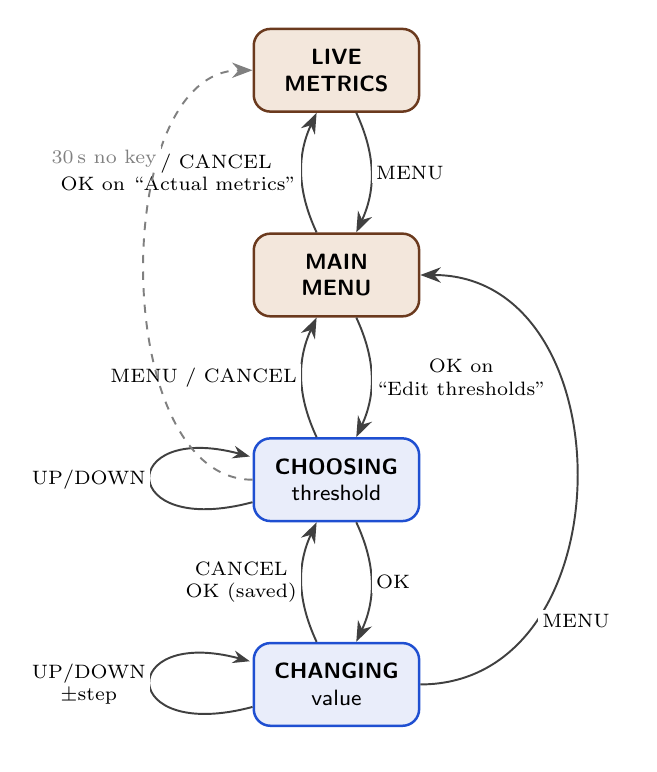
\begin{tikzpicture}[>=Stealth, every node/.style={font=\sffamily\scriptsize}]
  \node[st, minimum width=2.1cm] (n) at (0,0) {\textbf{LIVE}\\\textbf{METRICS}};
  \node[st, minimum width=2.1cm] (m) at (0,-2.6) {\textbf{MAIN}\\\textbf{MENU}};
  \node[stact, minimum width=2.1cm] (c) at (0,-5.2) {\textbf{CHOOSING}\\threshold};
  \node[stact, minimum width=2.1cm] (e) at (0,-7.8) {\textbf{CHANGING}\\value};
  \draw[tr] (n) to[bend left=25] node[lab,right] {MENU} (m);
  \draw[tr] (m) to[bend left=25] node[lab,left] {MENU / CANCEL\\OK on ``Actual metrics''} (n);
  \draw[tr] (m) to[bend left=25] node[lab,right] {OK on\\``Edit thresholds''} (c);
  \draw[tr] (c) to[bend left=25] node[lab,left] {MENU / CANCEL} (m);
  \draw[tr] (c) to[bend left=25] node[lab,right] {OK} (e);
  \draw[tr] (e) to[bend left=25] node[lab,left] {CANCEL\\OK (saved)} (c);
  \draw[tr] (e.east) to[out=0,in=0,looseness=1.3] node[lab,right,pos=0.25] {MENU} (m.east);
  \path (c) edge[tr, loop left] node[lab,left] {UP/DOWN} (c);
  \path (e) edge[tr, loop left] node[lab,left] {UP/DOWN\\$\pm$step} (e);
  \draw[tr, dashed, draw=gray] (c.west) to[out=180,in=180,looseness=0.9]
       node[lab,left,pos=0.7,text=gray] {30\,s no key} (n.west);
\end{tikzpicture}
\caption{Navigation between the screens. In every menu, 30\,s without a key press
returns to the live metrics.}
\label{fig:menu}
\end{figure}

\subsection{Buttons}
\begin{table}[h]
\centering\small
\caption{Role of the five buttons.}
\label{tab:buttons}
\begin{tabularx}{\columnwidth}{@{}l X@{}}
\toprule
Button & Action\\
\midrule
MENU   & open the main menu / go back to the previous level \\
OK     & enter the selected item / save the edited value \\
CANCEL & leave without saving \\
UP     & previous item, or $+$step while editing \\
DOWN   & next item, or $-$step while editing \\
\bottomrule
\end{tabularx}
\end{table}

Buttons are \textbf{debounced} in software (a level must be stable for 30\,ms). While
editing a value, holding UP or DOWN repeats the step every 120\,ms after 0.5\,s, and
10 times faster after 2\,s, so a value like the 15-minute cool-down (900\,s) can be
reached quickly. In the menus there is no auto-repeat, so a long press cannot skip
items by accident.

\subsection{Editable thresholds}
Table~\ref{tab:settings} lists the seven thresholds. A change is first a
\emph{draft}: it is applied only when OK is pressed, and only if the whole set of
settings stays valid; otherwise the screen shows \emph{Invalid value} and the old
value is kept. New values are used by the guards at the very next step, without any
restart.

\begin{table}[h]
\centering\small
\caption{Thresholds editable from the screen.}
\label{tab:settings}
\setlength{\tabcolsep}{3.5pt}
\begin{tabular}{@{}l r r r@{}}
\toprule
LCD label & Default & Range & Step\\
\midrule
Htarget (water<) & 35\,\% & 0--100\,\% & 1\\
Pump max time & 2\,s & 1--300\,s & 1\,s\\
Pump cooldown & 900\,s & 0--3600\,s & 5\,s\\
Tmin (heating) & 18\,$^\circ$C & $-10$--80 & 0.5\\
Tmax (cooling) & 28\,$^\circ$C & $-10$--80 & 0.5\\
Cooling min on & 60\,s & 0--600\,s & 5\,s\\
Tank empty < & 0 (raw) & 0--1023 & 1\\
\bottomrule
\end{tabular}
\end{table}

\subsection{Screen robustness}
Every fixed text (labels, messages, format strings) is stored in flash
(\code{PROGMEM}, \code{F()}, \code{PSTR()}) because the Uno has only 2\,KB of RAM.
Lines are always written as 16 characters padded with spaces instead of clearing the
screen, which avoids flicker. The I\textsuperscript{2}C bus has a 25\,ms timeout, so a
disconnected LCD can never freeze the controller: the automata keep running and the
screen is retried every 5\,s. Finally, the LCD is re-initialised 300\,ms after any
relay switches, and every 30\,s anyway (see Section~\ref{sec:difficulties}).

% =====================================================================
\section{Difficulties and how we handled them}\label{sec:difficulties}
% =====================================================================

\subsection{An extremely sensitive moisture sensor}
The resistive moisture sensor reacts to the water \emph{touching its legs}, not to
the average moisture of the soil. A single drop of water near the probe made the
reading jump very high, although the rest of the pot was still dry; a few minutes
later, when the water had spread, the value fell again. This had three consequences:
\begin{itemize}
  \item a ``water until the sensor says wet'' strategy would stop the pump almost
        immediately, or, depending on where the water falls, flood the pot;
  \item rates such as $\alpha$, $\beta$ or $b$ (Section~\ref{sec:modeling}) could not
        be measured from this signal;
  \item the reading also depends on the position and depth of the probe.
\end{itemize}
\textbf{What we did:} we water by short \emph{pulses} (2\,s) followed by a long
\emph{soak time} (15\,min cool-down) before the next decision, so the decision is
taken once the water has spread. We kept a single moisture threshold $H^*$ instead of
a band, because a moisture band would be fooled by the jumps. We also calibrated the
sensor with two points (Eq.~\ref{eq:calib}) and only power it while reading it,
which avoids corrosion of the legs, another source of drift.

\subsection{Inaccurate water-level sensor}
The resistive water-level strip gave inaccurate and unstable values: the reading
depends on the minerals in the water, on the oxidation of the copper tracks and on how
wet the strip still is above the water line. At one point it even read about 0 whatever
the water level. We wrote a dedicated diagnostic sketch, \code{WaterLevelTest.ino},
which prints the analog inputs with the probes powered and unpowered, to tell a wiring
error (signal on the wrong pin, no power, no ground) from a dead sensor.

\textbf{What we did:} we stopped trying to read a \emph{level} and only use the strip
as a binary \emph{tank OK / empty} safety signal compared with a threshold that can be
adjusted on the screen (\emph{Tank empty <}), so it can be recalibrated without
re-uploading the code. The sensor is powered (A2) only while it is read, like the
moisture probe.

\subsection{Testing could ruin the plant}
This was probably the hardest constraint. Testing an irrigation controller means
watering, and every test added water to the same pot: too many tests would drown the
plant and saturate the soil, which then needed hours or days to dry before the next
meaningful test. Identification experiments (pump for a known time, measure the
change) were especially destructive. We could not run as many tests as we wanted.

\textbf{What we did:}
\begin{itemize}
  \item tested the \emph{logic} without water as much as possible, by following the
        state changes in the serial log;
  \item made every threshold editable from the screen, so a test could be prepared
        (e.g.\ $H^*=0$ to disable watering, or short timers) without re-flashing;
  \item added a 30\,s start-up delay where nothing moves, to check all readings first;
  \item limited each watering to a short pulse, so a wrong decision costs only 2\,s of
        water;
  \item used small separate sketches (wiring check, calibration, water-level test)
        that keep every relay OFF.
\end{itemize}

\subsection{Finding a usable model}
As explained in Section~\ref{sec:modeling}, our continuous background pushed us first
towards transfer functions and then towards a hybrid automaton. Both failed for the same
reason: they need precise physical quantities that our sensors (and the risk to the
plant) did not let us measure. Accepting a purely discrete model with time in the
guards was a change of mindset, but it gave a controller that we can fully explain and
check.

\subsection{Other engineering issues}
\paragraph{Hardware integration and interference.} When a relay switched, the
voltage spike on the 5\,V line could knock the LCD out of step and fill it with random
symbols. We re-initialise the LCD shortly after each relay change and periodically.
The MAX6675 sometimes returned all zeros (which the library reports as 0.00\,$^\circ$C)
when its wiring or power was faulty; we treat this as an invalid reading, so the
temperature automaton goes to SENSOR\_ERROR instead of heating a greenhouse it believes
to be at 0\,$^\circ$C.

\paragraph{Timing without blocking.} Delays such as ``pump for 2\,s'' or ``wait
100\,ms for the probe'' cannot use \code{delay()}, which would freeze the buttons, the
screen and the other automaton. All timing is done by comparing \code{millis()} with
saved timestamps.

\paragraph{Memory.} With 2\,KB of RAM, every string and constant table had to be moved
to flash, and the automaton engine uses fixed arrays instead of dynamic containers.

\paragraph{Avoiding rapid switching.} Thresholds alone make actuators chatter when a
noisy measurement oscillates around them. The cool-down, the minimum fan time and the
$T_{low}$--$T_{high}$ band are our hysteresis mechanisms.

% =====================================================================
\section{Demonstration scenario}
% =====================================================================
During the demonstration the following behaviours can be shown, while following the
LCD and the serial log:
\begin{enumerate}
  \item \textbf{Start-up:} live metrics appear immediately; after 30\,s the log
        prints \emph{initial cool-down over -- automata running}.
  \item \textbf{Irrigation:} raise $H^*$ above the current moisture from the menu:
        the pump runs a 2\,s pulse (IDLE $\to$ IRRIGATING $\to$ IDLE), then waits for
        the cool-down.
  \item \textbf{Empty tank:} take the level sensor out of the water: the automaton
        goes to TANK\_EMPTY, the pump cannot start and the LCD shows \texttt{EMPTY}.
  \item \textbf{Heating / cooling:} set $T_{low}$ above or $T_{high}$ below the room
        temperature: the heater and fan (or the fan alone) start.
  \item \textbf{Sensor fault:} unplug the thermocouple: the LCD shows
        \texttt{T:--.-C}, the automaton goes to SENSOR\_ERROR and the heater and fan
        stop.
  \item \textbf{Invalid setting:} try to set $T_{low}\ge T_{high}$: the screen
        answers \emph{Invalid value}.
\end{enumerate}

% =====================================================================
\section{Conclusion and future work}\label{sec:conclusion}
% =====================================================================
We built Biodome, a working embedded controller that waters a plant and regulates the
temperature of a small greenhouse, with a screen and buttons to supervise and tune it.
The most important lesson of the project concerns \emph{modelling}: the models we knew
best (continuous dynamics, hybrid automata) were not the right ones for on/off
actuators and imprecise sensors. Extended finite-state machines, with time and
measurements inside the guards, gave a controller that is simple, deterministic,
safe by construction (safety transitions first, fail-safe states) and easy to adjust
on site.

\paragraph{Future work.}
\begin{itemize}
  \item Replace the resistive probes by a \emph{capacitive} moisture sensor (no
        corrosion, less sensitive to a single drop) and the level strip by a float
        switch or an ultrasonic sensor.
  \item Filter the moisture signal (median or moving average) and use several probes.
  \item Add a minimum ON time for heating, and an air-humidity sensor.
  \item With better sensors, return to an identified model ($\alpha$, $\beta$) and
        compare a PI controller with the automaton.
  \item Log the measurements to an SD card to study the greenhouse over several days.
  \item Move from the breadboard to a soldered PCB for reliability.
\end{itemize}

\bigskip
\infobox{Acknowledgements}{We thank our supervisor, Pr.\ BELAMFEDEL ALAOUI Sadek, for
the guidance throughout the project.}

\end{document}
